% This file is generated by the MATLAB m-file laprint.m. It can be included
% into LaTeX documents using the packages graphicx, color and psfrag.
% It is accompanied by a postscript file. A sample LaTeX file is:
%    \documentclass{article}\usepackage{graphicx,color,psfrag}
%    \begin{document}% This file is generated by the MATLAB m-file laprint.m. It can be included
% into LaTeX documents using the packages graphicx, color and psfrag.
% It is accompanied by a postscript file. A sample LaTeX file is:
%    \documentclass{article}\usepackage{graphicx,color,psfrag}
%    \begin{document}% This file is generated by the MATLAB m-file laprint.m. It can be included
% into LaTeX documents using the packages graphicx, color and psfrag.
% It is accompanied by a postscript file. A sample LaTeX file is:
%    \documentclass{article}\usepackage{graphicx,color,psfrag}
%    \begin{document}% This file is generated by the MATLAB m-file laprint.m. It can be included
% into LaTeX documents using the packages graphicx, color and psfrag.
% It is accompanied by a postscript file. A sample LaTeX file is:
%    \documentclass{article}\usepackage{graphicx,color,psfrag}
%    \begin{document}\input{Noise}\end{document}
% See http://www.mathworks.de/matlabcentral/fileexchange/loadFile.do?objectId=4638
% for recent versions of laprint.m.
%
% created by:           LaPrint version 3.16 (13.9.2004)
% created on:           16-Jul-2010 14:14:49
% eps bounding box:     15 cm x 11.25 cm
% comment:              
%
\begin{psfrags}%
\psfragscanon%
%
% text strings:
\psfrag{s03}[t][t]{\color[rgb]{0,0,0}\setlength{\tabcolsep}{0pt}\begin{tabular}{c}$f/\mathrm{Hz}$\end{tabular}}%
\psfrag{s04}[b][b]{\color[rgb]{0,0,0}\setlength{\tabcolsep}{0pt}\begin{tabular}{c}$S_n(f)/\mathrm{Hz}^{-1}$\end{tabular}}%
%
% xticklabels:
\psfrag{x01}[t][t]{$10^{-6}$}%
\psfrag{x02}[t][t]{$10^{-5}$}%
\psfrag{x03}[t][t]{$10^{-4}$}%
\psfrag{x04}[t][t]{$10^{-3}$}%
\psfrag{x05}[t][t]{$10^{-2}$}%
\psfrag{x06}[t][t]{$10^{-1}$}%
\psfrag{x07}[t][t]{$10^{0}$}%
\psfrag{x08}[t][t]{$10^{1}$}%
%
% yticklabels:
\psfrag{v01}[r][r]{$10^{-41}$}%
\psfrag{v02}[r][r]{$10^{-39}$}%
\psfrag{v03}[r][r]{$10^{-37}$}%
\psfrag{v04}[r][r]{$10^{-35}$}%
\psfrag{v05}[r][r]{$10^{-33}$}%
\psfrag{v06}[r][r]{$10^{-31}$}%
\psfrag{v07}[r][r]{$10^{-29}$}%
\psfrag{v08}[r][r]{$10^{-27}$}%
%
% Figure:
\resizebox{12cm}{!}{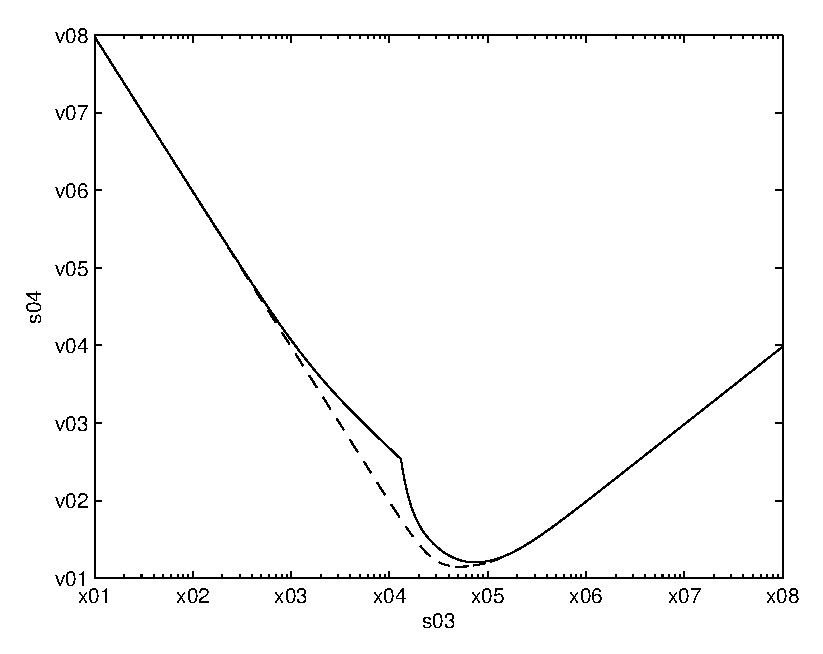
\includegraphics{Noise.eps}}%
\end{psfrags}%
%
% End Noise.tex
\end{document}
% See http://www.mathworks.de/matlabcentral/fileexchange/loadFile.do?objectId=4638
% for recent versions of laprint.m.
%
% created by:           LaPrint version 3.16 (13.9.2004)
% created on:           16-Jul-2010 14:14:49
% eps bounding box:     15 cm x 11.25 cm
% comment:              
%
\begin{psfrags}%
\psfragscanon%
%
% text strings:
\psfrag{s03}[t][t]{\color[rgb]{0,0,0}\setlength{\tabcolsep}{0pt}\begin{tabular}{c}$f/\mathrm{Hz}$\end{tabular}}%
\psfrag{s04}[b][b]{\color[rgb]{0,0,0}\setlength{\tabcolsep}{0pt}\begin{tabular}{c}$S_n(f)/\mathrm{Hz}^{-1}$\end{tabular}}%
%
% xticklabels:
\psfrag{x01}[t][t]{$10^{-6}$}%
\psfrag{x02}[t][t]{$10^{-5}$}%
\psfrag{x03}[t][t]{$10^{-4}$}%
\psfrag{x04}[t][t]{$10^{-3}$}%
\psfrag{x05}[t][t]{$10^{-2}$}%
\psfrag{x06}[t][t]{$10^{-1}$}%
\psfrag{x07}[t][t]{$10^{0}$}%
\psfrag{x08}[t][t]{$10^{1}$}%
%
% yticklabels:
\psfrag{v01}[r][r]{$10^{-41}$}%
\psfrag{v02}[r][r]{$10^{-39}$}%
\psfrag{v03}[r][r]{$10^{-37}$}%
\psfrag{v04}[r][r]{$10^{-35}$}%
\psfrag{v05}[r][r]{$10^{-33}$}%
\psfrag{v06}[r][r]{$10^{-31}$}%
\psfrag{v07}[r][r]{$10^{-29}$}%
\psfrag{v08}[r][r]{$10^{-27}$}%
%
% Figure:
\resizebox{12cm}{!}{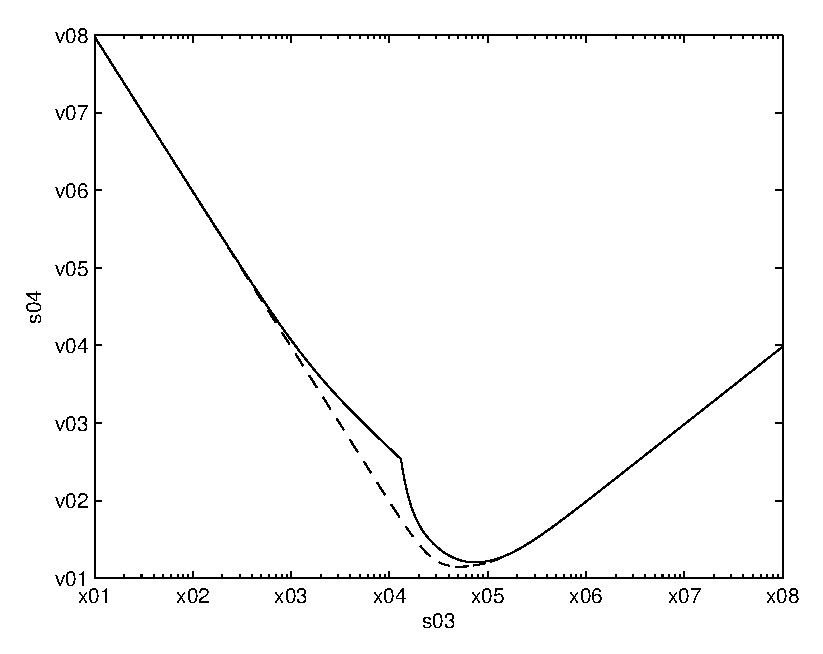
\includegraphics{Noise.eps}}%
\end{psfrags}%
%
% End Noise.tex
\end{document}
% See http://www.mathworks.de/matlabcentral/fileexchange/loadFile.do?objectId=4638
% for recent versions of laprint.m.
%
% created by:           LaPrint version 3.16 (13.9.2004)
% created on:           16-Jul-2010 14:14:49
% eps bounding box:     15 cm x 11.25 cm
% comment:              
%
\begin{psfrags}%
\psfragscanon%
%
% text strings:
\psfrag{s03}[t][t]{\color[rgb]{0,0,0}\setlength{\tabcolsep}{0pt}\begin{tabular}{c}$f/\mathrm{Hz}$\end{tabular}}%
\psfrag{s04}[b][b]{\color[rgb]{0,0,0}\setlength{\tabcolsep}{0pt}\begin{tabular}{c}$S_n(f)/\mathrm{Hz}^{-1}$\end{tabular}}%
%
% xticklabels:
\psfrag{x01}[t][t]{$10^{-6}$}%
\psfrag{x02}[t][t]{$10^{-5}$}%
\psfrag{x03}[t][t]{$10^{-4}$}%
\psfrag{x04}[t][t]{$10^{-3}$}%
\psfrag{x05}[t][t]{$10^{-2}$}%
\psfrag{x06}[t][t]{$10^{-1}$}%
\psfrag{x07}[t][t]{$10^{0}$}%
\psfrag{x08}[t][t]{$10^{1}$}%
%
% yticklabels:
\psfrag{v01}[r][r]{$10^{-41}$}%
\psfrag{v02}[r][r]{$10^{-39}$}%
\psfrag{v03}[r][r]{$10^{-37}$}%
\psfrag{v04}[r][r]{$10^{-35}$}%
\psfrag{v05}[r][r]{$10^{-33}$}%
\psfrag{v06}[r][r]{$10^{-31}$}%
\psfrag{v07}[r][r]{$10^{-29}$}%
\psfrag{v08}[r][r]{$10^{-27}$}%
%
% Figure:
\resizebox{12cm}{!}{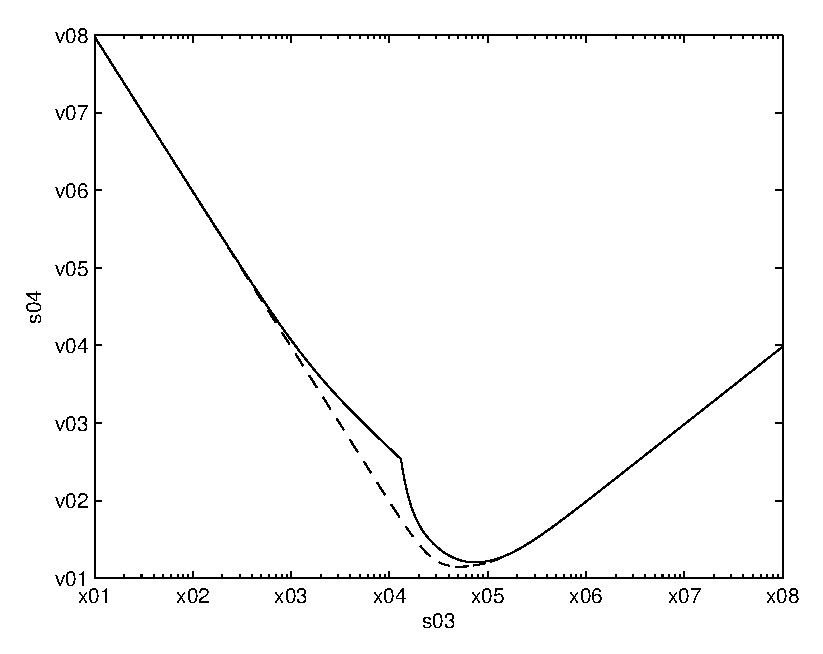
\includegraphics{Noise.eps}}%
\end{psfrags}%
%
% End Noise.tex
\end{document}
% See http://www.mathworks.de/matlabcentral/fileexchange/loadFile.do?objectId=4638
% for recent versions of laprint.m.
%
% created by:           LaPrint version 3.16 (13.9.2004)
% created on:           16-Jul-2010 14:14:49
% eps bounding box:     15 cm x 11.25 cm
% comment:              
%
\begin{psfrags}%
\psfragscanon%
%
% text strings:
\psfrag{s03}[t][t]{\color[rgb]{0,0,0}\setlength{\tabcolsep}{0pt}\begin{tabular}{c}$f/\mathrm{Hz}$\end{tabular}}%
\psfrag{s04}[b][b]{\color[rgb]{0,0,0}\setlength{\tabcolsep}{0pt}\begin{tabular}{c}$S_n(f)/\mathrm{Hz}^{-1}$\end{tabular}}%
%
% xticklabels:
\psfrag{x01}[t][t]{$10^{-6}$}%
\psfrag{x02}[t][t]{$10^{-5}$}%
\psfrag{x03}[t][t]{$10^{-4}$}%
\psfrag{x04}[t][t]{$10^{-3}$}%
\psfrag{x05}[t][t]{$10^{-2}$}%
\psfrag{x06}[t][t]{$10^{-1}$}%
\psfrag{x07}[t][t]{$10^{0}$}%
\psfrag{x08}[t][t]{$10^{1}$}%
%
% yticklabels:
\psfrag{v01}[r][r]{$10^{-41}$}%
\psfrag{v02}[r][r]{$10^{-39}$}%
\psfrag{v03}[r][r]{$10^{-37}$}%
\psfrag{v04}[r][r]{$10^{-35}$}%
\psfrag{v05}[r][r]{$10^{-33}$}%
\psfrag{v06}[r][r]{$10^{-31}$}%
\psfrag{v07}[r][r]{$10^{-29}$}%
\psfrag{v08}[r][r]{$10^{-27}$}%
%
% Figure:
\resizebox{12cm}{!}{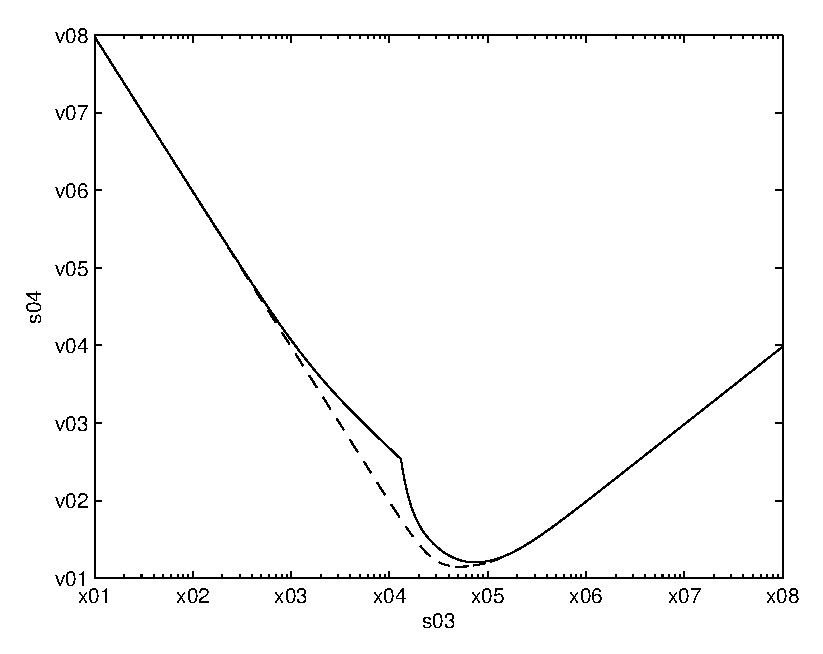
\includegraphics{Noise.eps}}%
\end{psfrags}%
%
% End Noise.tex
